
\section{Introdução}

Este documento serve o propósito de documentar o estudo e desenvolvimento levado a cabo no projecto integrado da unidade curricular de sistemas distribuídos.

As próximas secções desta introdução introduzem conceitos e tecnologias utilizadas com o objectivo de suportar as análises posteriores no relatório.

\subsection{Ruby}

\subsection{Message oriented middleware (MOM)} 

Entende-se por \textit{message oriented middleware} (MOM) como um método de comunicação entre componentes de sistemas distribuídos.


\begin{description}
  \item[Assincrono] \hfill \\
  	Permite que um cliente não bloqueie enquanto espera por resposta.
  \item[Second]
  \item[Third] The third etc \ldots
\end{description}

No contexto deste relatório entede-se por MOM como uma camada de comunicação que permite a várias aplicações comunicar ignorando as especificidades de cada uma.

% Websockets

\subsection{Introdução a \textit{websockets}}

A conceção inicial da web focou apenas apenas comunicação cliente-servidor num sentido apenas. Actualmente com o HTML5 está a procurar corrigir-se esta entrave, contudo ainda muitos projectos utilizam \textit{long-polling} para simular a comunicação cliente-servidor.

Actualmente os browsers são actualizados regularmente e suportam a API de comunicação do HTML5.

\subsubsection{\textit{Long pulling}}

\begin{figure}[H]
\centering
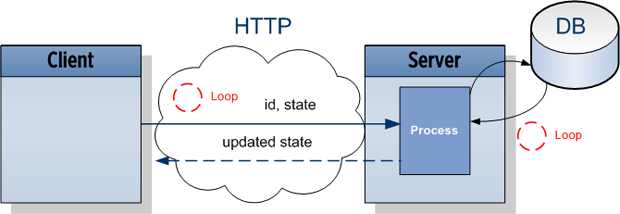
\includegraphics[width=0.9\textwidth]{longpolling-architecture.png}
\caption{Esquema de \textit{long pulling}}
\label{fig:long_pulling}
\end{figure}

Um cliente (browser) envia por HTTP um pedido para o servidor com o identificador do utilizador (por exemplo) e do estado actual. No servidor é criado um processo que repetidamente verifica na base de dados se existe um estado novo. Quando existe um novo estado o cliente recebe e envia um novo pedido ao servidor.

\subsubsection{\textit{Server-Sent Events}}

\begin{figure}[H]
\centering
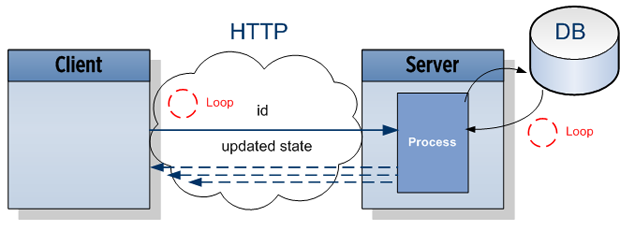
\includegraphics[width=0.9\textwidth]{sse-architecture.png}
\caption{Esquema de \textit{server-sent events}}
\label{fig:long_pulling}
\end{figure}

Um cliente (browser) faz um pedido ao servidor por HTTP. O servidor responde com o último estado na base de dados. O cliente recebe a resposta e em três segundos (por exemplo) envia um novo pedido.

\subsubsection{Websockets}

\begin{figure}[H]
\centering
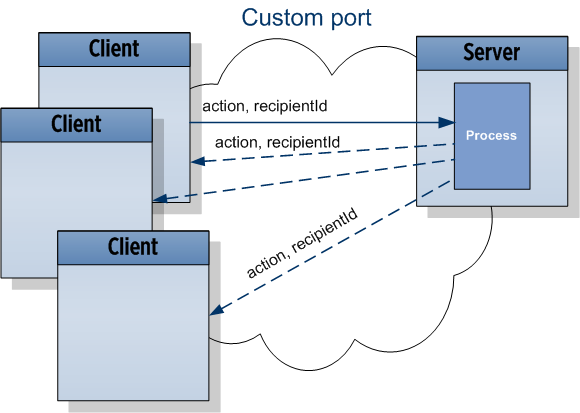
\includegraphics[width=0.9\textwidth]{websocket-architecture.png}
\caption{Esquema de \textit{websockets}}
\label{fig:long_pulling}
\end{figure}

Um cliente notifica o servidor de websockets de um evento. O servidor imediamente notifica todos os clientes ativos do evento. Este processo pode envolver filtros e subscrição de eventos.